\documentclass[a4paper,11pt]{article}

\usepackage{fullpage}
\usepackage{color}
\usepackage{hyperref}
\usepackage{amsmath}
\usepackage{amssymb}
\usepackage{tikz}
\usepackage{tabularx}
\usepackage{booktabs}
\usepackage{amsmath}
\usepackage{multirow}
\usepackage{layouts}
\usepackage{array}
\usepackage{pgf}
\usepackage{tikz}
\usepackage{amssymb}
\usepackage{graphics}
\usepackage{eucal}
\usepackage{ifthen}
\usepackage{ifpdf}
\usepackage{lmodern}
\usepackage{amsthm}
\usetikzlibrary{positioning}

\hypersetup{
  colorlinks,%
    citecolor=black,%
    filecolor=black,%
    linkcolor=black,%
    urlcolor=mygreylink     % can put red here to visualize the links
}

\definecolor{hlcolor}{rgb}{1, 0, 0}
\definecolor{mygrey}{gray}{.85}
\definecolor{mygreylink}{gray}{.30}
\textheight=8.6in
\raggedbottom
\addtolength{\oddsidemargin}{-0.375in}
\addtolength{\evensidemargin}{0.375in}
\addtolength{\textwidth}{0.5in}
\addtolength{\topmargin}{-.375in}
\addtolength{\textheight}{0.75in}


\newcommand{\resheading}[1]{{\large \colorbox{mygrey}{\begin{minipage}{\textwidth}{\textbf{#1 \vphantom{p\^{E}}}}\end{minipage}}}}

\newcommand{\mywebheader}{
  \begin{tabular}{@{}p{5in}p{4in}}
  {\resheading{Assignment 3: Multi Agent Planning and Learning}} & {\Large 19 October, 2012}\\\vspace{0.2cm}
  \end{tabular}}

\begin{document}


\begin{center}
{\LARGE \textbf{Autonomous Agents}}\\ [1em]
\end{center}
\mywebheader

\begin{center}
{\Large By:} \\ \vspace{0.1cm}
{\Large Paris Mavromoustakos} \\  \vspace{0.1cm}
{\Large Georgios Methenitis} \\ \vspace{0.1cm}
{\Large Patrick de Kok} \\ \vspace{0.1cm}
{\Large Marios Tzakris}
\end{center}




\section{Introduction}

In this last assignment, we added multiple predators to the environment, while making the prey intelligent, therefore, harder to catch. Our previous implementations already considered the prey to be an agent, for that reason we only made minor changes to our prey's functions, allowing it to use learning methods just like the predators. The prey will now move with equal probability towards all directions, always, with a chance to trip, it stays in the same position independently from the action that it chooses, otherwise one predator would never be able to catch it.

What we also changed is that the prey and predator(s) move simultaneously, in a single time-step. That means, the agents can be next to each other and swap positions, without considering their next move to be "safe" or not.

Last, we now consider this implementation to be a zero-sum Markov game, because predators are going to receive a negative $-10$ reward if they crash into each other, while the prey will be receiving a positive $+10$ reward. Beside that, the predators will receive reward $+10$ for catching the prey which gets $-10$ for getting caught.



\section{Exercise 1}

In the first exercise, we use the $11 \times 11$ grid where we add a prey and more than one predators. Our implementation requests the number of predators as input from the user, initializes the prey at position $<5,5>$ and puts the predators in random positions. 

The agents then move randomly on the grid until two predators move into the same position (Collision) or a predator catches the prey (Catch). These two are the only possible absorbing states. We should note, that, if two predators collide and the prey is caught in the same time-step, the predators' collision is more "important" and defines the reward distribution.


\subsection{Results}
Table~\ref{table:multirandom}, presents the results we had in the first part of the exercise. In this random implementation predator(s) and prey always act randomly. Adding more predators to this particular case o random actions by all agents does reduce the number of steps needed to catch the prey but dramatically increases the number of collisions between predators. In the last column of the table we present the average number of needed time-steps for the predator(s) to catch the prey. The results of this random implementation are exactly as we expected.
\begin{table}[h]
\begin{center}
\caption{Multiple Agents' Random Implementation}
\begin{tabular}{c c c c} 
\hline\hline               
\textbf{\small{Number of Predators}} & \textbf{\small{Total No. of Collisions}} & \textbf{\small{Total No. of Catches}} & \textbf{\small{Average Step No. until Catch}} \\  
\hline
1 & 0 & 500 & 185\\ 
2 & 175 & 325  & 59\\
3 & 255 & 245   & 27\\
4 & 292 & 208 & 15 \\ 
\end{tabular}
\label{table:multirandom} 
\end{center} 
\end{table} 

\section{Exercise 2}

\subsection{Independent Q-Learning}
In the first part of the second exercise, we made both prey and predators "intelligent" by implementing the \textit{Q-Learning} algorithm on every agent. That means that all agents save and use their own Q(s,a) table, from which they choose the next action using $\epsilon$-greedy action selection.

All predator now, have their own learning algorithm which will lead them to choose worthy actions for their own success. Considering the reward function discussed above, we expect a cooperative behavior among the predators, as all predators will get a positive reward in cases that a predator manage to catch the prey. For the prey, we only expect to be smart enough and to avoid being caught. In this implementation, $P_{trip}$ (the chance of the prey tripping) becomes important, as it allows the predators to move faster than the prey, thus getting a bigger chance to catch it. If this probability was not taken into consideration, the prey would always run away, especially when it competes only with one predator.

We have seen, that independent \textit{Q-Learning} has very nice results in this multi-agent framework. However, the space complexity of this algorithm makes it computationally intractable in environments that there is a big number of agents. For example, in our problem and a number of four agents, each agent is going to need to save in its Q-table up to $1.071.794.405$ state-action pairs, given that each agent has $121$ possible states, and the selected agent has $5$ actions. Table~\ref{table:complexity}, presents how the number grows exponentially as the number of agents goes up in our state space. We were able to implement independent \textit{Q-Learning} even for four agents, three predators and one prey, considering prey's position always at $<5,5>$, and transform its action to predators' movement. Running the same algorithm for five agents was unfeasible, due to memory limitations.


\begin{table}[h]
\begin{center}
\caption{Multiple Agents' Random Implementation}
\begin{tabular}{c l} 
\hline\hline               
\textbf{\small{Number of Agents}} & \textbf{\small{\# State-Action}} \\  
\hline
1 & $605$\\ 
2 & $73.205$\\
3 & $8.857.805$\\
4 & $1.071.794.405$\\
5 & $129.687.123.005$\\
6 & $1.569214188 \times 10^{13}$\\
\end{tabular}
\label{table:complexity} 
\end{center} 
\end{table} 

\subsubsection{Results}
Figure~\ref{q2}, illustrates our results in independent \textit{Q-Learning}
\begin{figure}[t!]
  \centering
    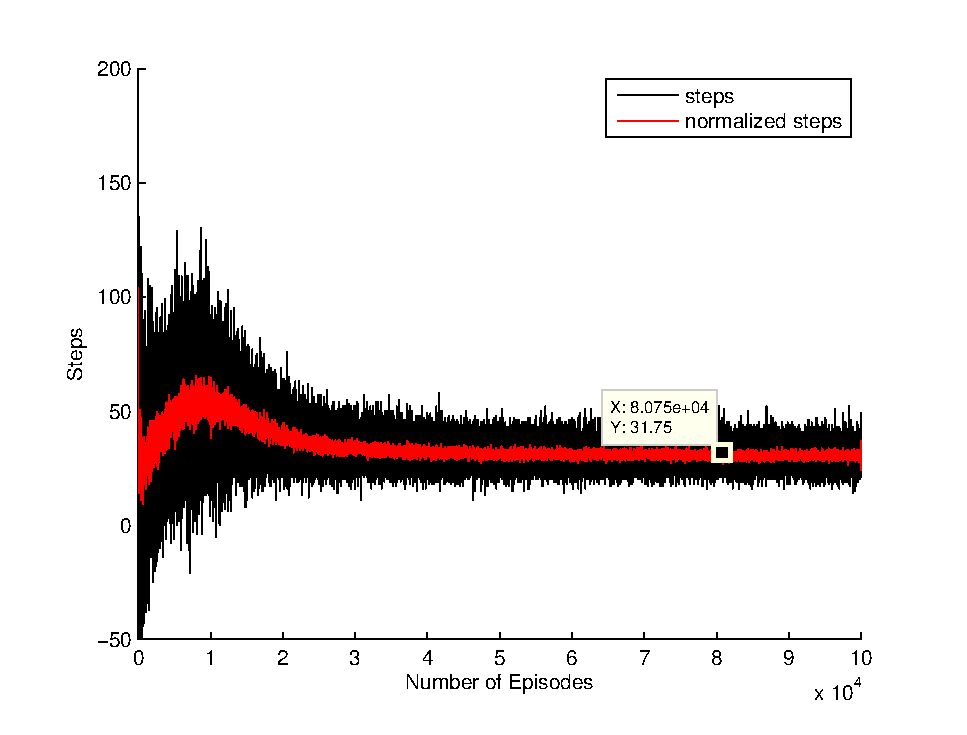
\includegraphics[width=0.49\textwidth]{figures/q207.eps}\	
    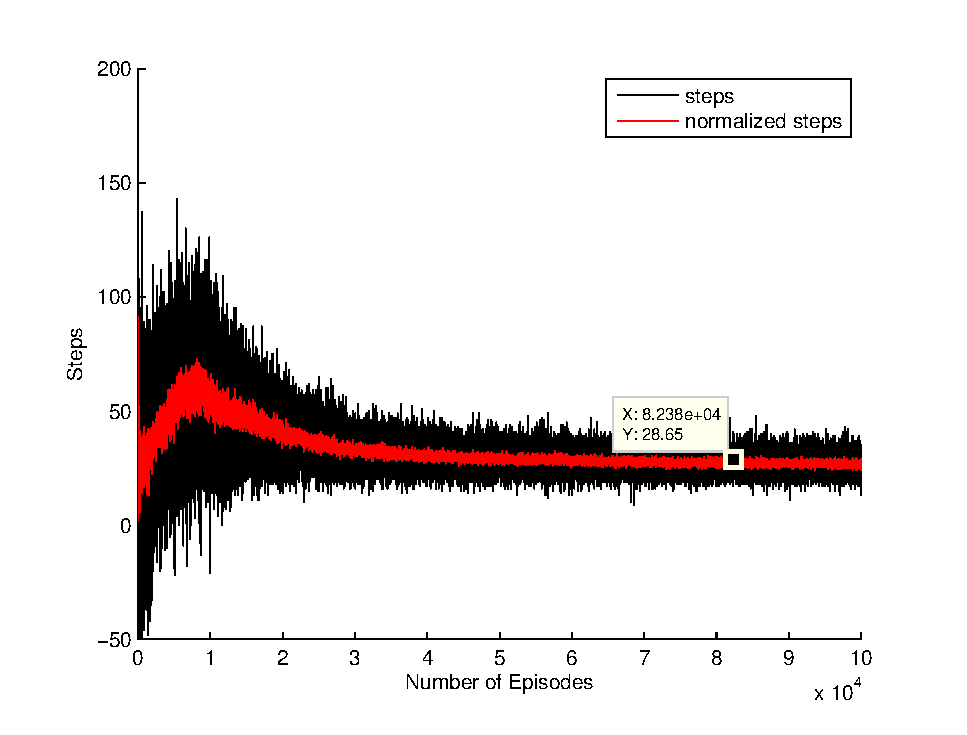
\includegraphics[width=0.49\textwidth]{figures/q205.eps} \\
    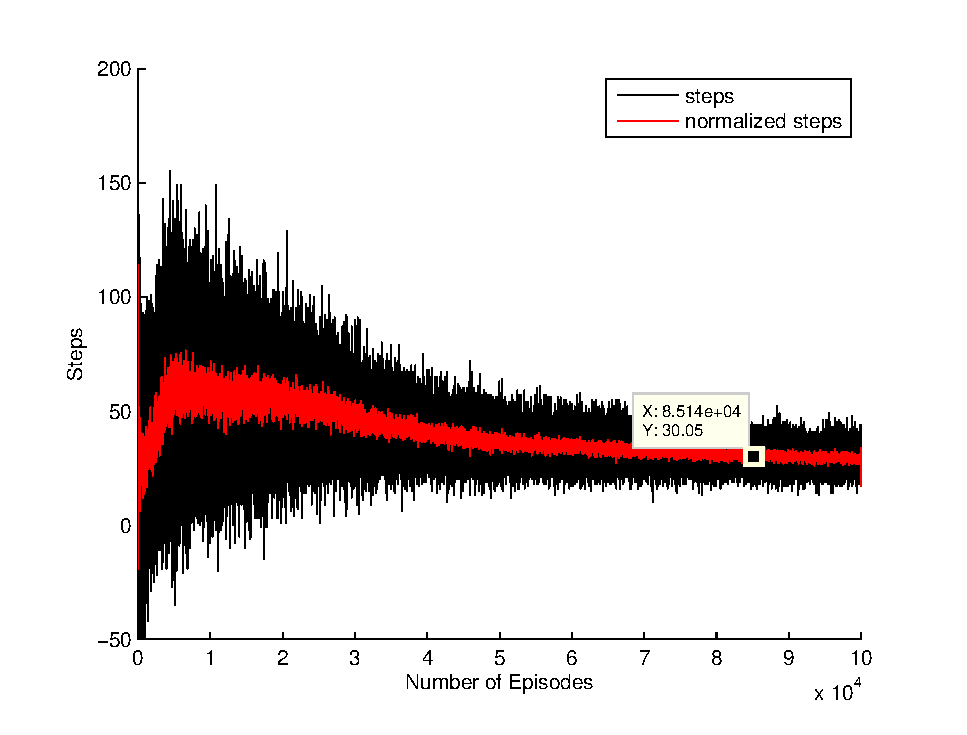
\includegraphics[width=0.5\textwidth]{figures/q202.eps} \\
    \caption{A picture of a gull.}
    \label{q2}
\end{figure}

Figure~\ref{qtest}, 
\begin{figure}[t!]
  \centering
    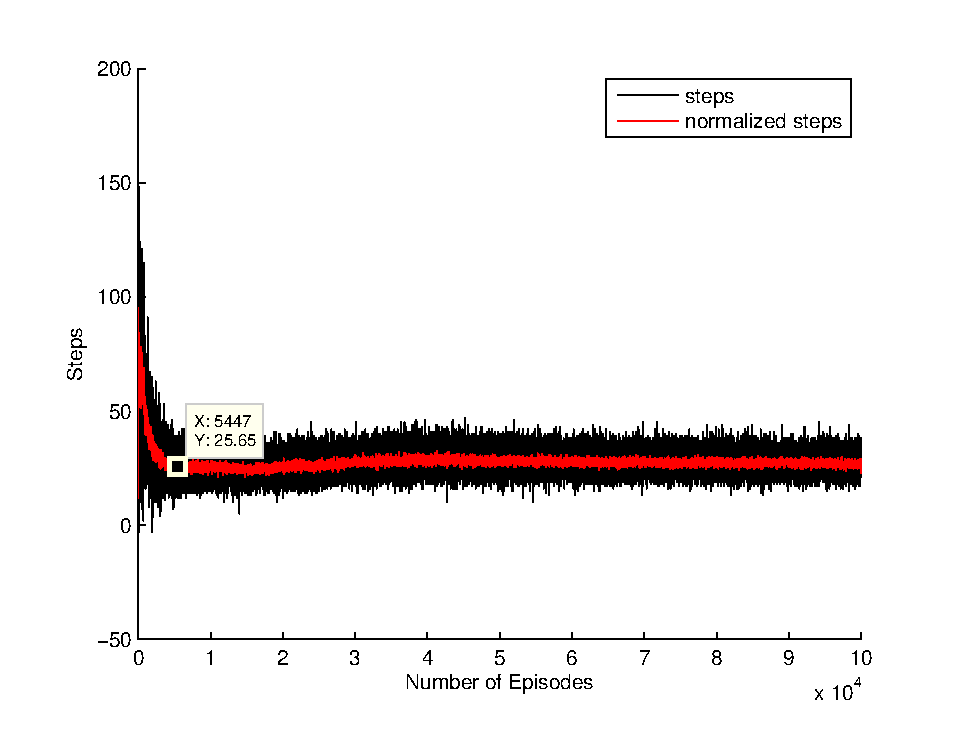
\includegraphics[width=0.49\textwidth]{figures/q2init.eps}\	
    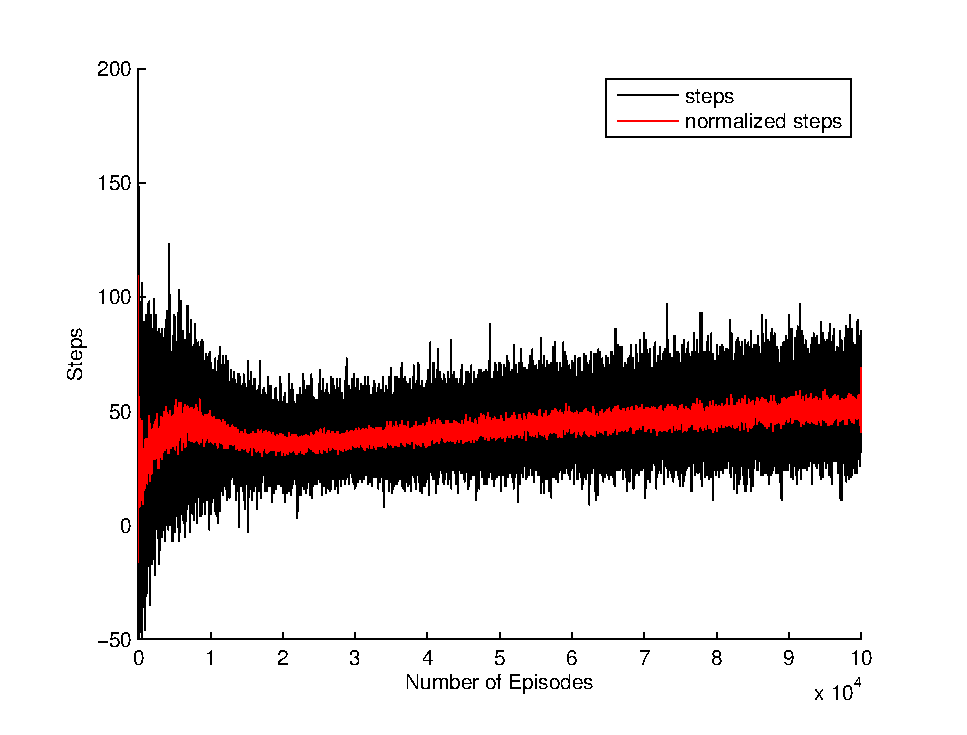
\includegraphics[width=0.49\textwidth]{figures/q2learnfast.eps}
    \caption{A picture of a gull.}
    \label{qtest}
\end{figure}


\subsection{Minimax Q-Learning}

In the second part of the first exercise we implemented the \textit{minimax Q-Learning} algorithm, as described in the paper: \textit{"Markov games as a framework for multi-agent reinforcement learning" by M.L. Littman, 1994}.

\subsubsection{Description}
First, the algorithm discussed in that paper is only described in a zero-sum two player markov game. The obvious goal of both agents is to maximize their expected sum of discounted rewards, just like in an MDP. However, this algorithm discriminates the two agents by introducing a single reward function $R(s,a,o)$, which each agent tries to maximize and the other one (opponent) tries to minimize it. So, for example, when the game is in state $s$, the predator will consider the prey will pick the optimal action $o$ which means the worst action for its opponent. As a consequence, the predator will choose the next possible action $s$ that maximizes its reward, always considering the worst case scenario. On the other hand, the prey will consider the predator picking the next possible action that is optimal. Generally, it is a fact that in the minimax-Q algorithm each agent considers its opponent to be optimal (picking the optimal actions each time), and defines its next action according to that. 

The \textit{minimax Q-Learning} algorithm consists of three parts: 	Initialisation, choosing the next action and learning. Each agent initializes its own $Q[s,a,o]$ table, with initial value, $1$. For each possible state s, it also initializes the state value $V[s]$ table with initial value of $1$, as well. The probability between all the possible actions $a \in A$ deriving from each state $s$ is distributed equally, with $P(s,a_{i}) = 1/|A|$ $\forall a_i \in A$, and is also saved in the $\pi$-table, $pi[s,a]$. Learning rate $\alpha$ is also initialized as $1$ and will descend as the steps in each episode goes on. That means, the agents learn based on their immediate past in the beginning of the algorithm, but they consider their past to become more important in the next stages as they do not learn if learning rate becomes very low.

After the initialization of the data, each agent will have to choose its next action. That depends on a variable $\epsilon$, so as, agents choose the action with maximum probability in the $pi[s,a]$ table with probability $1-\epsilon$, but they choose a random action among the possible ones with probability $\epsilon$. This is very similar to $\epsilon$-greedy action selection, but this time, the action is chosen based on its probability of being chosen and not on its expected reward. The learning part of the algorithm is described below:

\begin{itemize}
\item After receiving reward $R_t$ for moving from state $s$ to $s'$ , via action $a$ and opponent's action $o$,
\[
Q_{t+1}[s,a,o] = (1-\alpha)\times Q_t[s,a,o] + \alpha \times (r + \gamma \times V[s'])
\]

\item We used linear programming to find $pi[s,.]$ such that:
\[
pi[s,.] = \arg\max_{pi'[s,.]} {(\min_{o'} \sum_{a'} (pi[s,a'] \times Q[s,a',o']))}
\]
In fact we need to maximize what our opponent agent wants to minimize. The maximization term goes to the probabilities of choosing our set of actions, given that our opponent is going to minimize it. For the linear programming we used $6$ variables. One for the opponent's minimization $m$, and the remaining $5$ for our actions, $p_1$,$p_2$,\ldots,$p_5$. Linear programming needs constraints in order to maximize the given linear combination of variables. Our main function to maximize was $f(m)$, and the constraints were:
\begin{itemize}
\item $ \sum_{i}{p_i} = 1.0$
\item $ p_i \geq 0.0$
\item $ \sum_{a'} (pi[s,a'] \times Q[s,a',o']) \geq m$, $\forall o' \in O$
\end{itemize}
\item The value of the state s will be equal with the maximized value of variable from the linear program m: $V[s] = m$
\item Learning rate will be always decayed in each update: $\alpha = \alpha \times decay$. $decay \in (0,1)$ is the variable we use to reduce the value of $\alpha$.
\end{itemize}
\subsection{Results}


\section{WoLF-PHC}
In the final part of the exercise we chose to implement \textit{Wolf-Policy Hill Climbing}. This algorithm is described in detail in the slides of the Autonomous Agents course. In addition, the paper \textit{``Efficient Learning in Games'', by Raghav Aras, Alain Dutech and Francois Charpillet}, was really useful for us in order to implement this algorithm.

The general idea behind this algorithm is that, agent chooses its action by its $\pi$-table in respect to the probability of each action. Next, agent updates its Q-table:
\[
Q_{t+1}(s,a) \leftarrow (1-\alpha)Q_{t}(s,a)+\alpha(r + \gamma \max_{a'}Q(s',a'))
\]
Next, agent has to update its average policy. Every state has a counter which indicated the times that was visited by the agent in the past. Using this counter, agent, is able to update the value of the its current state's policy for all actions:
\[
\bar{\pi}(s,b) \leftarrow \bar{\pi}(s,b) + \cfrac{1}{V} (\pi(s,b) - \bar{\pi}(s,b)), \forall b
\]
,where $V$ is the number of visits in this state. A big difference from the other learning algorithms is on the policy update. In general this algorithm uses two variables to change the probability of choosing the taken action. $\delta_{win}$, $\delta_{lose}$, the first one is used whenever agent chose an action which was better than the average policy and the second for the opposite case. This unique way to update the policy being followed by the agent is the main characteristic of this algorithm.
\subsection{Results}

\section{Conclusion}
In this last assignment of the Autonomous Agents course, we implemented and experimented on different learning algorithms that can be used in multi-agent frameworks. We comprehend how more than one agents can explode the space complexity of these specific algorithms, considering that fact, we can understand the reason why planning and learning in multi-agent system have triggered a great research interest the last decade.


\end{document}